\documentclass{beamer}
\usetheme{Lab2C}

\usepackage{graphicx}
\usepackage{subcaption}
\usepackage{amsthm}
\usepackage{mathtools}
\DeclarePairedDelimiter\abs{\lvert}{\rvert}
\DeclarePairedDelimiter\norm{\lVert}{\rVert}
\DeclarePairedDelimiter\inner{\langle}{\rangle}
\def\P{\mathcal{P}}
%further improvement
%background intro added Chen Chuan's work
%simulation add hierarchical method
%find suitable dataset to apply info-clustering
%Yang Li's suggestion: compared with other clustering method, the threshold is the same or not
%early stopping technique, complexity from n -> log(n)
\title{An information-theoretic approach to cluster random variables}
\author{Feng Zhao\inst{1} \and Fei Ma\inst{2} \and Shao-Lun Huang\inst{2} \and Lin Zhang\inst{2}}
\institute{\inst{1}Dept. of Electronic Engineering, Tsinghua University
\and \inst{2}Tsinghua-Berkeley Shenzhen Institute, Tsinghua University}
\date{\today}
\begin{document}
\begin{frame}
	\titlepage
\end{frame}
\section*{Outline}
\begin{frame}
	\tableofcontents
\end{frame}

\section{Introduction}
\subsection{Overview of existing clustering method}
\begin{frame}
\frametitle{Existing clustering method}
\begin{figure}
    \centering
    \begin{subfigure}[b]{0.3\textwidth}
        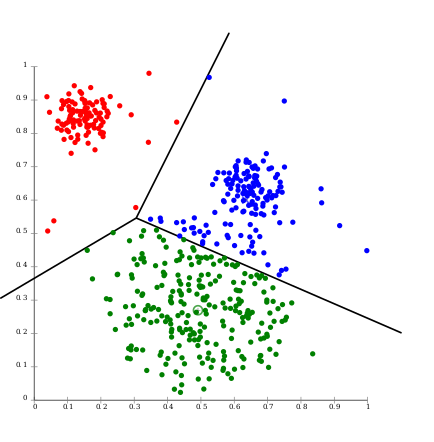
\includegraphics[width=\textwidth]{pic/kmeans.png}
        \caption{KMeans}
    \end{subfigure}~
    \begin{subfigure}[b]{0.3\textwidth}
        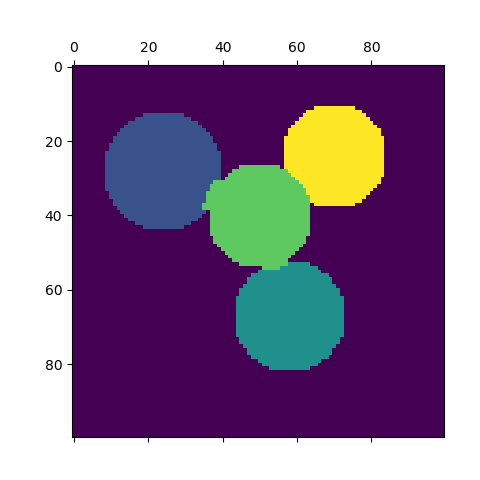
\includegraphics[width=\textwidth]{pic/spectral_clustering.png}
        \caption{Spectral clustering}
    \end{subfigure}
    ~ %add desired spacing between images, e. g. ~, \quad, \qquad, \hfill etc. 
    %(or a blank line to force the subfigure onto a new line)
    \begin{subfigure}[b]{0.3\textwidth}
        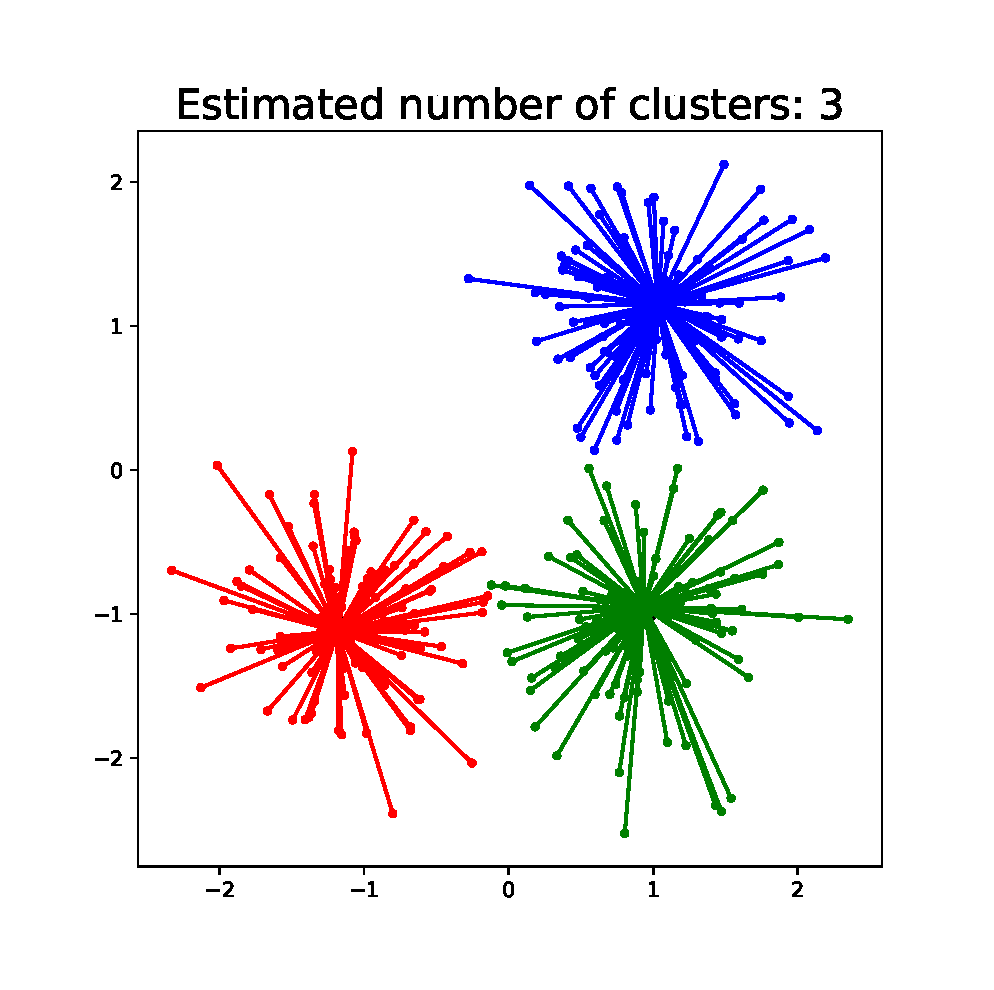
\includegraphics[width=\textwidth]{pic/affinity_propagation.eps}
        \caption{Affinity propagation}
    \end{subfigure}
\end{figure}
\end{frame}

\subsection{Mutual Similarity and its extension}
\begin{frame}
\begin{block}{mutual similarity}
\begin{itemize}
\item Gaussian kernel $ \exp({-\gamma \norm{p_1 - p_2}^2})$
\item mutual information $I(X;Y)$ for random variables
\end{itemize}
\end{block}

\begin{definition}[Multivariate information]
Given an undirected Graph $G(V, E)$, with vertex as data point, edge weight as mutual similarity, the multivariate information $I(Z_V)$
\begin{align}
I(Z_V) & = \min_{\mathcal{P} \in \Pi'(V)} I_{\mathcal{P}}(Z_V) \\
\label{eq:newDef}  I_{\mathcal{P}}(Z_V) & = {1 \over 2 ( \abs{\mathcal{P}} - 1) } \sum_{\substack{i\in C, j \not\in C\\ C\in \mathcal{P}}} w_{ij}
\end{align}
\end{definition}
\end{frame}
\begin{frame}
\frametitle{Illustrative example}
\begin{columns}
\column{5cm}
\begin{figure}
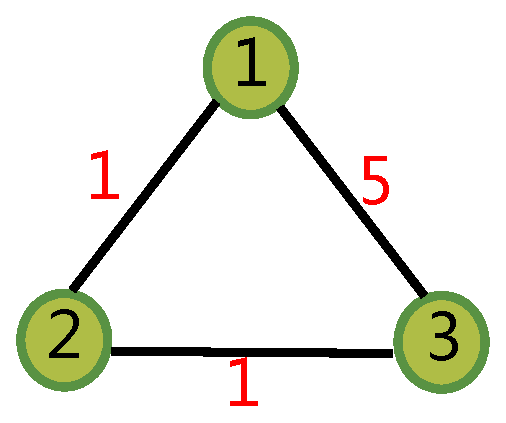
\includegraphics[width=4cm]{pic/example.eps}
\end{figure}
\column{5cm}
\begin{align*}
I_{\{1\},\{2\},\{3\}}(Z_{\{1,2,3\}}) & = 3.5 \\
I_{\{1,3\},\{2\}}(Z_{\{1,2,3\}}) & = 2 \\ 
I_{\{1,2\},\{3\}}(Z_{\{1,2,3\}}) & = 6 \\ 
I_{\{1\},\{2,3\}}(Z_{\{1,2,3\}}) & = 6 \\ 
\Rightarrow I(Z_{\{1,2,3\}}) & = 2 \\
\end{align*}
\begin{equation*}
I(Z_{\{1,3\}}) = 5, I(Z_{\{1,2\}}) = 1
\end{equation*}
\end{columns}
\end{frame}
%\section{B matrix and its relationship with multivariate mutual information}

\begin{frame}{Hierachical clustering method}
To cluster $Z_1, Z_2, \dots, Z_{\abs{V}}$ for threshold $\gamma$.
The clusters are:
\begin{equation}
C_{\gamma}(Z_V) = \textrm{maximal}\{ B \subseteq V \vert \abs{B} > 1, I(Z_B) > \gamma \}
\end{equation}
More specificly:
\begin{equation*}
C_{\gamma}(Z_V) = \begin{cases}
\{V\} & \gamma < \gamma_1 \\
C_{\gamma_i}(Z_V) & \gamma \in [\gamma_i, \gamma_{i+1}), 1\leq i < N \\
\emptyset & \gamma \geq \gamma_N
\end{cases}
\end{equation*}
$\gamma_i$: \alert{critical values}
\end{frame}
\begin{frame}
\frametitle{Illustrative example}
\begin{columns}
\column{4cm}
\begin{figure}
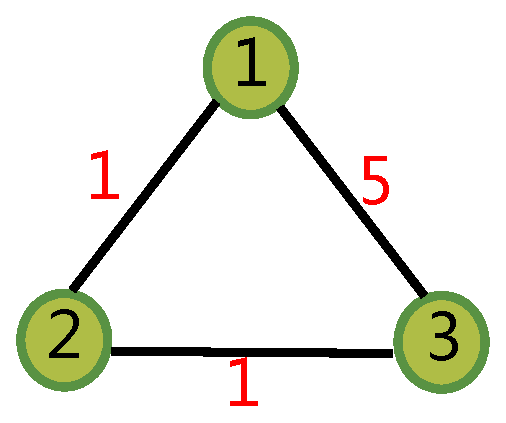
\includegraphics[width=4cm]{pic/example.eps}
\end{figure}
\column{6cm}
\begin{equation*}
I(Z_{\{1,2,3\}}) = 2, I(Z_{\{1,3\}}) = 5
\end{equation*}
\begin{equation*}
C_{\gamma}(Z_{\{1,2,3\}}) = \begin{cases}
\{1,2,3\} & \gamma \in (-\infty, 2) \\
\{1, 3\} & \gamma \in [2, 5) \\
\emptyset & \gamma \in [5, \infty)
\end{cases}
\end{equation*}
\end{columns}
\end{frame}
\section{Info-Cluster Algorithms}
\begin{frame}
\begin{definition}[graph cut function]
$C$ is a subset of $V$:
\begin{align}
f(C) & ={1 \over 2} \sum_{i\in C, j \not\in C} w_{ij} \\
f[\P] & = \sum_{C \in \P} f(C)
\end{align}
\end{definition}
\begin{theorem}
\begin{equation}\label{eq:hLambda}
h(\lambda) = \min_{\P \in \Pi(V)} \{ f[\P] - \abs{\P}\lambda \}
\end{equation} piesewise linear about $\lambda$. 
$\gamma_i$: turning points; $\P_i$ corresponding partation. $C_{\gamma_i}(Z_V)$: non-singleton element of $\P_i$.
\end{theorem}
\end{frame}
\begin{frame}
\frametitle{Illustrative Example}
\begin{columns}
\column{5cm}
\begin{figure}
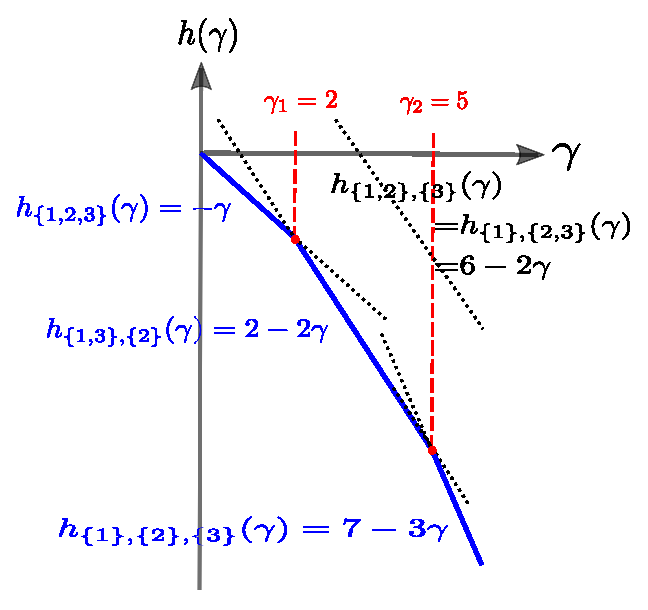
\includegraphics[width=5cm]{pic/dt.eps}
\caption{Dilworth truncation of $f(\P)$}
\end{figure}
\column{5cm}
\begin{align*}
h(\lambda)  & = \min_{\P} h_{\lambda}(\P) \\
h_{\lambda}(\P) & = f[\P] - \abs{\P}\lambda
\end{align*}
\begin{align*}
\P_0  & = \{\{1,2,3\}\} \\
\P_1  & = \{\{1,3\},\{2\}\} \\
\P_2  & = \{\{1\},\{2\},\{3\}\} 
\end{align*}

\end{columns}
\end{frame}
\begin{frame}
\begin{columns}
\column{5cm}
\begin{figure}[!ht]
\centering
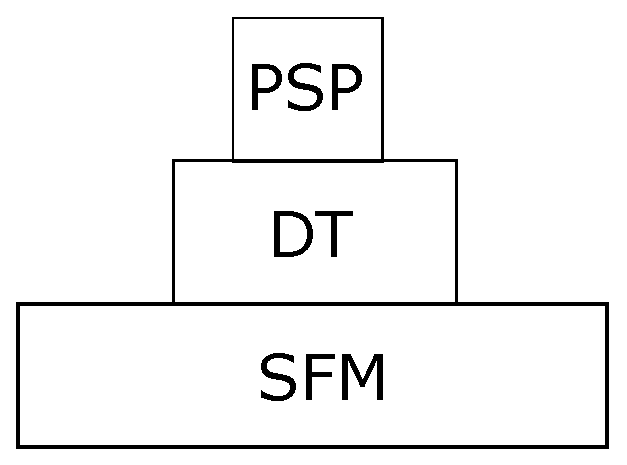
\includegraphics[width=5cm]{pic/pyramid.eps}
\caption{pyramid structure of info-clustering algorithm}\label{fig:ps}
\end{figure}
\column{5cm}
\begin{enumerate}
\item principal sequence of partation: $\P_i$
\item Dilworth truncation: evaluate $h(\lambda)$
\item submodular function minimization
\end{enumerate}
SFM converted to graph max flow.

Time Complexity: $\abs{V}^2 \mathrm{MF}(G(V,E))$
% For push-relabel algorithm, \mathrm{MF}(G(V,E)) = \abs{V}^2 E
\end{columns}
\end{frame}
\section{Numerical Results}
\begin{frame}
\begin{figure}[!ht]
\centering
\begin{subfigure}{\textwidth}
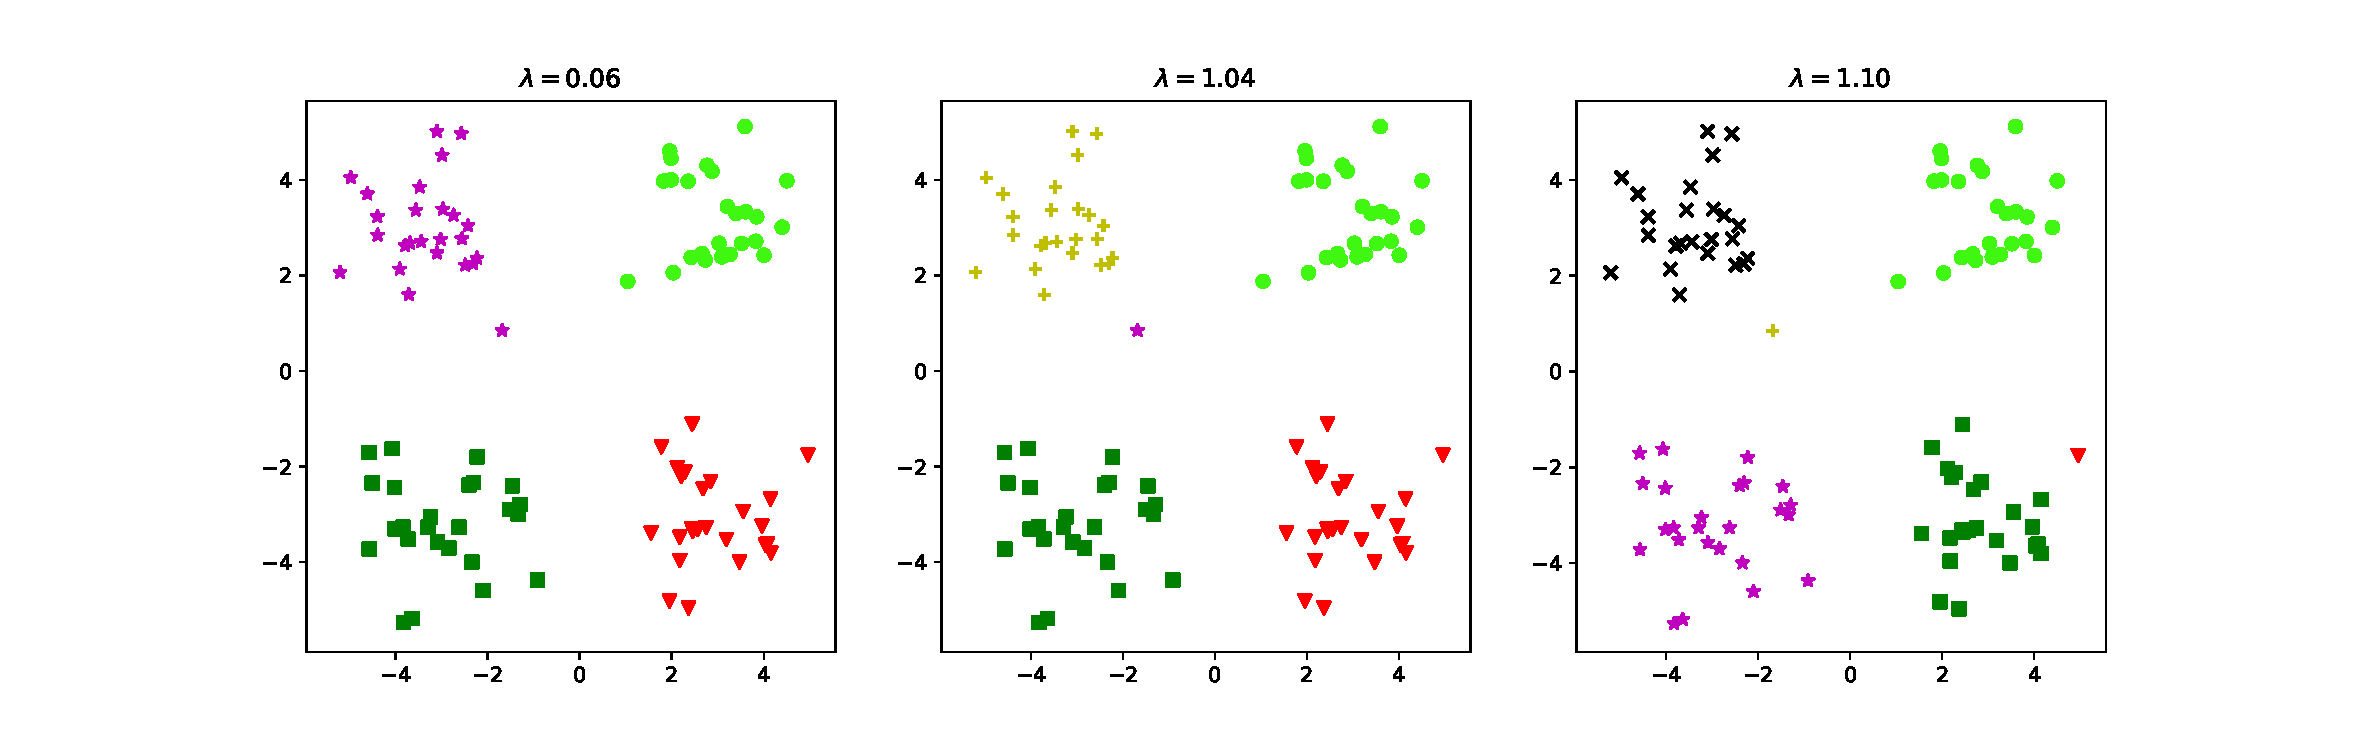
\includegraphics[width=12cm]{pic/4part.eps}
\caption{Illustrative example from four Gaussians}\label{fig:4p}
\end{subfigure}
\begin{subfigure}{\textwidth}
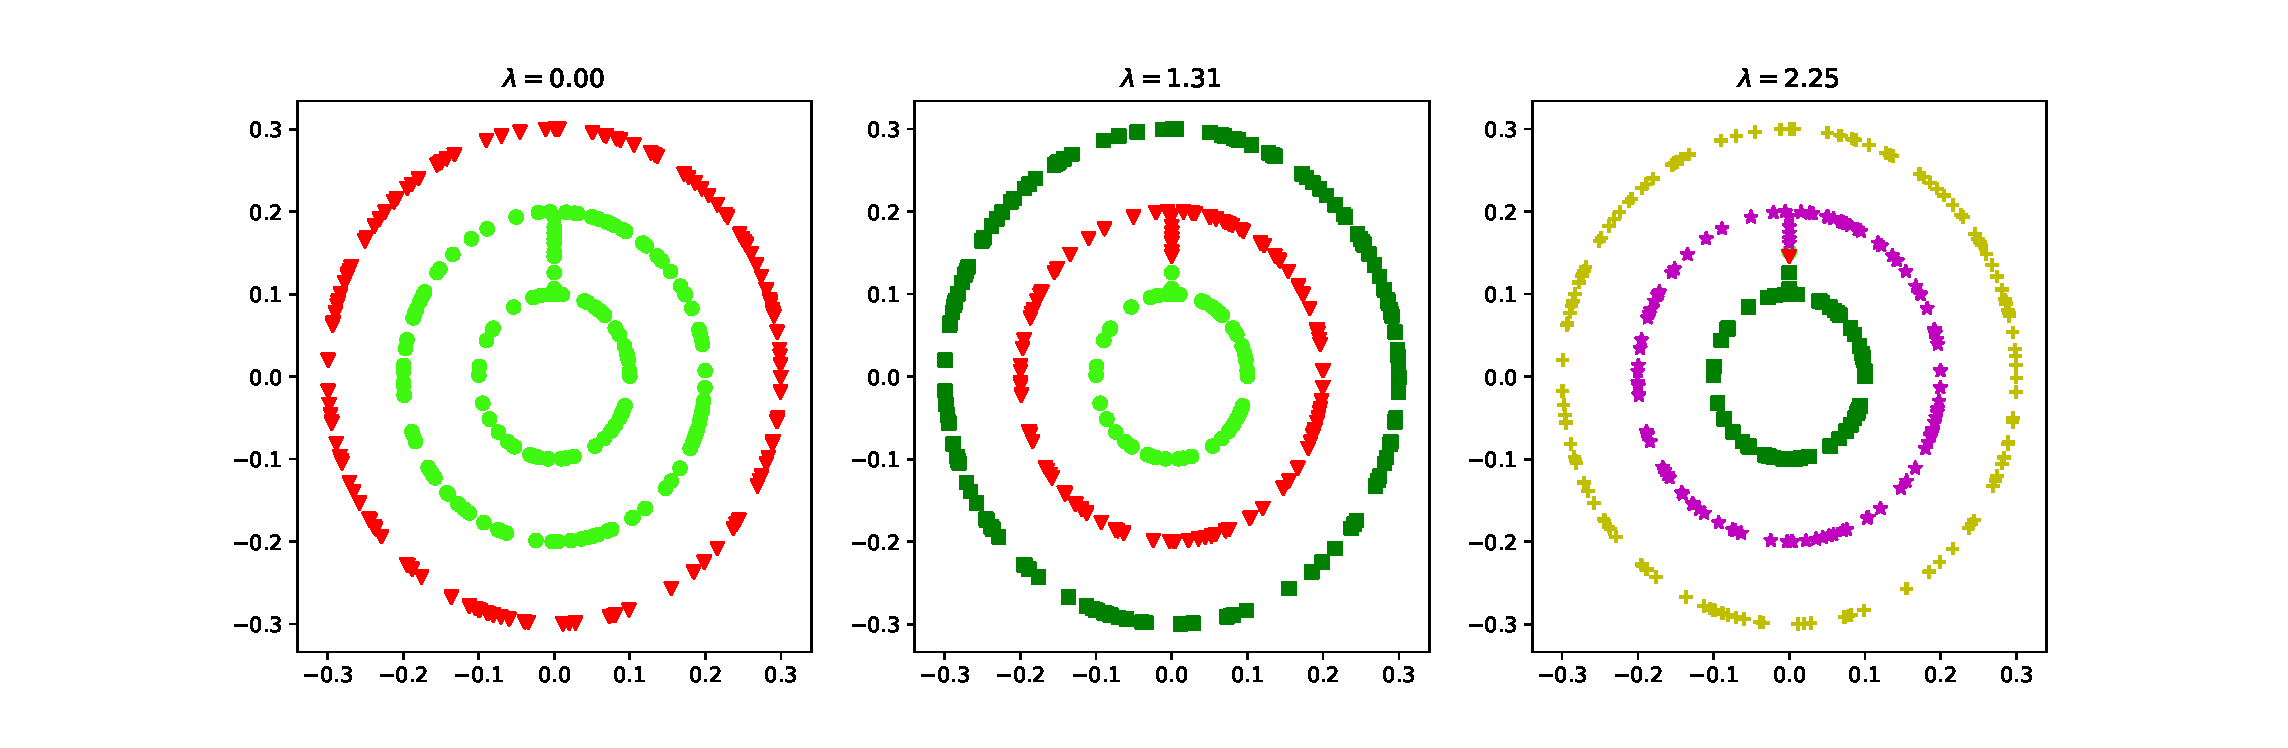
\includegraphics[width=12cm]{pic/3circle.eps}
\caption{Illustrative example from three circles}\label{fig:3c}
\end{subfigure}
\end{figure}
\end{frame}
\begin{frame}
\frametitle{empirical comparision}
\begin{table}[!ht]
\centering
\begin{tabular}{lrrrrr}
\hline
                      &   Gaussian &   Circle &   Iris &   Glass &   Libras \\
\hline
 k-means              &          1 &     0.02 &   0.59 &    0.21 &     0.33 \\
 spectral clustering  &          1 &     1    &   0.65 &    0.15 &     0.38 \\
 affinity propagation &          1 &     0    &   0.63 &    0.19 &     0.3  \\
 info-clustering      &          1 &     0.81 &   0.56 &    0.3  &     0.13 \\
\hline
\end{tabular}
\caption{clustering accuracy for info-clustering and existing algorithms}
\end{table}
\end{frame}
\section{Conclusion and Contribution}
\begin{frame}
\frametitle{Conclusion}
\begin{itemize}
\item propose multivariate information, used in info-clustering method
\item implement info-clustering algorithm
\item competitive with existing algorithms in some dataset
\end{itemize}
\end{frame}
\section{Reference}
\begin{frame}
\frametitle{Further Reading}
\begin{thebibliography}{9}
\bibitem{ic} Chung Chan, \newblock Info-Clustering: A Mathematical Theory for Data Clustering
\newblock  IEEE Transactions on Molecular, Biological and Multi-Scale Communications, June 2016
\bibitem{pin}  Chung Chan, \newblock Info-Clustering: An Efficient Algorithm by Network Information Flow
\newblock 2017 Information Theory and Applications Workshop (ITA)
\bibitem{mac} Kiyohito Nagano \newblock Minimum Average Cost Clustering \newblock NIPS 2010
\end{thebibliography}
\end{frame}
\end{document}